% Indicate the main file. Must go at the beginning of the file.
% !TEX root = ../main.tex

%%%%%%%%%%%%%%%%%%%%%%%%%%%%%%%%%%%%%%%%%%%%%%%%%%%%%%%%%%%%%%%%%%%%%%%%%%%%%%%%
% 04_discussion
%%%%%%%%%%%%%%%%%%%%%%%%%%%%%%%%%%%%%%%%%%%%%%%%%%%%%%%%%%%%%%%%%%%%%%%%%%%%%%%%


\section{Discussion}
\label{discussion}

\subsection{Best Model Performance}

The best performing model achieved a reasonable high accuracy of 0.92. The validation
metrics loss and accuracy are shown in \autoref{fig:best_model_training_metrics}
suggest a reasonable progress during the fitting process. Since they both are not
all the way flattening out, it might even be possible to further improve the model
using the same architecture and hyperparameters by training it for more epochs.
This could be achieved by using a higher value for the \texttt{patience} parameter --
the next value to be tested could be 20 instead of 10.

\begin{figure}[H]
    \centering
    \captionsetup{width=0.8\linewidth}
    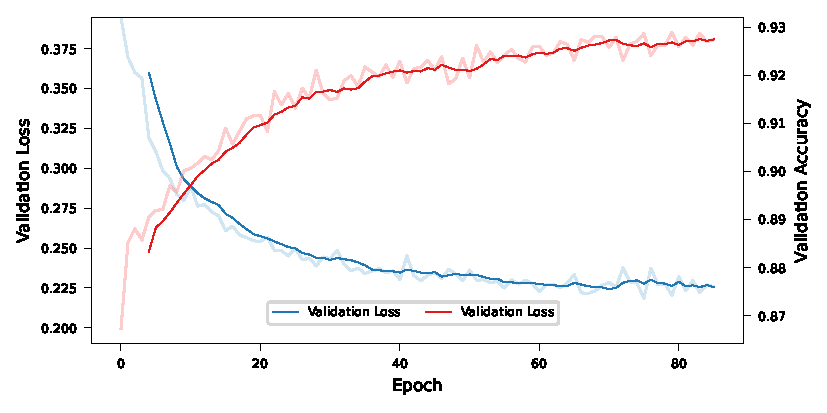
\includegraphics{figures/best_model_training_metrics.pdf}
    \caption{Validation loss and accuracy for the best model.}
    \label{fig:best_model_training_metrics}
\end{figure}

The accuracy per class, shown in \autoref{fig:best_model_accuracy_per_category}
does align with expectations. Classes like Building, GreenAreas, RoadAsphalt, Forrest,
and MadowPasture are predicted with high accuracy. While classes, where there is
very little data available like WaterBasin or classes where the data is more vague
like ConstructionSites are predicted with lower accuracy.

\subsection{Hyperparameter Tuning}

The hyperparameter tuning process was successful in finding the best hyperparameters
within the grid search. It is hard to argue for clear tendencies what works best.
\autoref{fig:hp_tuning_boxplot} shows a lower \texttt{learning\_rate} seems to work better and that
the augmentation makes a significant difference for \texttt{weight\_decay = 0.1} values.
The grid of evaluated hyperparameters was rather limited dew to limited computational
resources in the remaining time. A more extensive search could potentially lead to
even better results. What might really be worth trying is to test for even smaller
values of \texttt{learning\_rate} and to use the other options for the data augmentation --
pixel- and channel noise in different combinations.

\subsection{Comparing the Results to the GIS Approach}